\documentclass[journal]{IEEEtai}

\usepackage[colorlinks,urlcolor=blue,linkcolor=blue,citecolor=blue]{hyperref}

\usepackage{color,array}
\usepackage{cite}
\newcommand{\tabitem}{~~\llap{\textbullet}~~}
\usepackage{graphicx}
\usepackage{tikz}
\usepackage{caption}
\usepackage{comment}

\usepackage{booktabs, makecell, multirow, tabularx}
\newcolumntype{C}{>{\centering\arraybackslash}X} % centered version of "X" type
\newcommand\mcx[1]{\multicolumn{1}{C}{#1}}
\setlength{\extrarowheight}{1pt}
\usepackage{stfloats}
\usepackage{siunitx}
\usepackage{caption}
\newcommand{\ap}[1]{AP\textsubscript{#1}}
\newcommand{\apavg}[0]{AP\textsubscript{\(\!\varnothing\)}}


%% \jvol{XX}
%% \jnum{XX}
%% \paper{1234567}
%% \pubyear{2020}
%% \publisheddate{xxxx 00, 0000}
%% \currentdate{xxxx 00, 0000}
%% \doiinfo{TQE.2020.Doi Number}

\newtheorem{theorem}{Theorem}
\newtheorem{lemma}{Lemma}
\setcounter{page}{1}
%% \setcounter{secnumdepth}{0}



\usepackage[backend=bibtex, style=ieee]{biblatex}
\addbibresource{library}

\begin{document}


\title{Bankruptcy prediction in Colombian case, using multilayer perceptron trained with memetic algorithm} 


\author{ Iván andrés Trujillo \IEEEmembership{PUJ MINTA}}

\author{Student:Iván Andrés Trujillo Abella,\\

\\
\\

Proffesors: Eliana María González Neira \& Gabriel Mauricio Zambrano Rey}
\maketitle

\begin{abstract}
Literature about Bankruptcy prediction is still incipient, therefore this work try to fill this gap by using machine learning  and metaheuristics techniques to find an optimal set of  weights in a MLP model.
\end{abstract}


\begin{IEEEkeywords}
Machine learning, Bankruptcy, Metaheuristics, Evolutionary Algorithms, Local Search, Memetic algorithms, Neural Networks, Multilayer Perceptron.
\end{IEEEkeywords}





\section{Information(Data)}

Data was retrieved from SIS by the period 2016-2019, classifying as bankrupt all Small and Medium Enterprises(SMEs) firms  that enter in process of insolvency.


\subsection{Event definition}


The event was determined as firms that enter of one year to another in a insolvency process.

To model the phenomena were used  financial ratios of one and two year before of the occurrence of the event. For instance, those firms that have a normal state in 2018 and enter in insolvency process in 2019 the  financial ratios of 2018 and 2017 to model the event in 2019. 

For those firms that not present the event(controls) were used the mean of financial ratio by its period of activity. For instance, $j$ firm enter to the database in 2017 and not present the event then were used the mean of the financial ratios for the period (2017 - 2019).
\subsection{Exclusion criteria}

\begin{itemize}

\item Were excluded financial information present in a date different to December 31 of each year.

\item Were excluded from database firms that declared in a preoperative condition each year (this and the former criteria give us unique firms).


\item Were excluded from database those firms that present the event for the initial year (2016). 


\item Were excluded firms that present missing  values in financial ratios using to prediction. 
\end{itemize}


\section{Description of data}

To describe categorical data were used absolute and relative frequencies. The numerical variables were describe with mean and standard deviation if the variable is normally distributed, otherwise were used median and 25\% and 75\% percentile.


To compare the financial ratios and determine if there are significance difference  among bankrupt and no-bankrupt firms, we used t-test or wilcoxon rank sum test if the variable is normal or not respectively, to test normally we used  shapiro-wilk test. To determine if there are independence among the event and categorical variables the $\chi^{2}$ test was used. 






\section{Modelling prediction}

The models used to benchmark were: Decision tree, logistic regression and multilayer perceptron.


\subsection{Train and test}

We used 65\% to train and 35\% to test.


\subsection{Hyperparameter tunning}

\subsection{Balance data}


We used udersampling.



\section{Results}




\usetikzlibrary{shapes.geometric, arrows}

\tikzstyle{startstop} = [rectangle, rounded corners, 
minimum width=3cm, 
minimum height=1cm,
text centered, 
draw=black, 
fill=red!30]

\tikzstyle{io} = [ rectangle, minimum width=3cm, 
minimum height=1cm, text centered, 
draw=black, fill=white!30]

\tikzstyle{process} = [rectangle, 
minimum width=3cm, 
minimum height=1cm, 
text centered, 
text width=3cm, 
draw=black, 
fill=white!30]

\tikzstyle{decision} = [rectangle, 
minimum width=3cm, 
text width = 3cm,
minimum height=1cm, 
text centered, 
draw=black, 
fill=gray!30]

\tikzstyle{arrow} = [thick,->,>=stealth]

\begin{document}

\begin{figure}[h]
\begin{tikzpicture}[node distance=2cm]
\node (box1) [process] {Initial database  
N = 27,210 
Bankrupt = 1279};
\node (text1) [decision, left of=box1, xshift = -3cm] {Unique firms by period};

\node (box2) [process, below of=box1] {N = 26,702 
Bankrupt = 771
};

\node (text2) [decision, left of=box2, xshift = -3cm] {Without firms that bankrupt in 2016};




\node (box3) [process, below of=box2] {N = 17613 
Bankrupt = 328};


\node (text3) [decision, left of=box3, xshift = -3cm] {Firms that have complete variables to modelling};


\node (box4) [process, below of=box3] {N = 17613 
Bankrupt = 318};


\node (text4) [decision, left of=box4, xshift = -3cm] {Firms with valid financial ratios};

	
\draw [arrow] (text1) -- (box1);
\draw [arrow] (box1) -- (box2);
\draw [arrow] (text2) -- (box2);
\draw [arrow] (box2) -- (box3);
\draw [arrow] (text3) -- (box3);
\draw [arrow] (box3) -- (box4);
\draw [arrow] (text4) -- (box4);
\end{tikzpicture}
\end{figure}


For the period (2016-2019) 700 firms were found as 



According to the following figure the spearman coefficient show the monotocity relationship among the predictors.

\begin{figure}[h]
\caption{Spearman correlation in predictor variables}
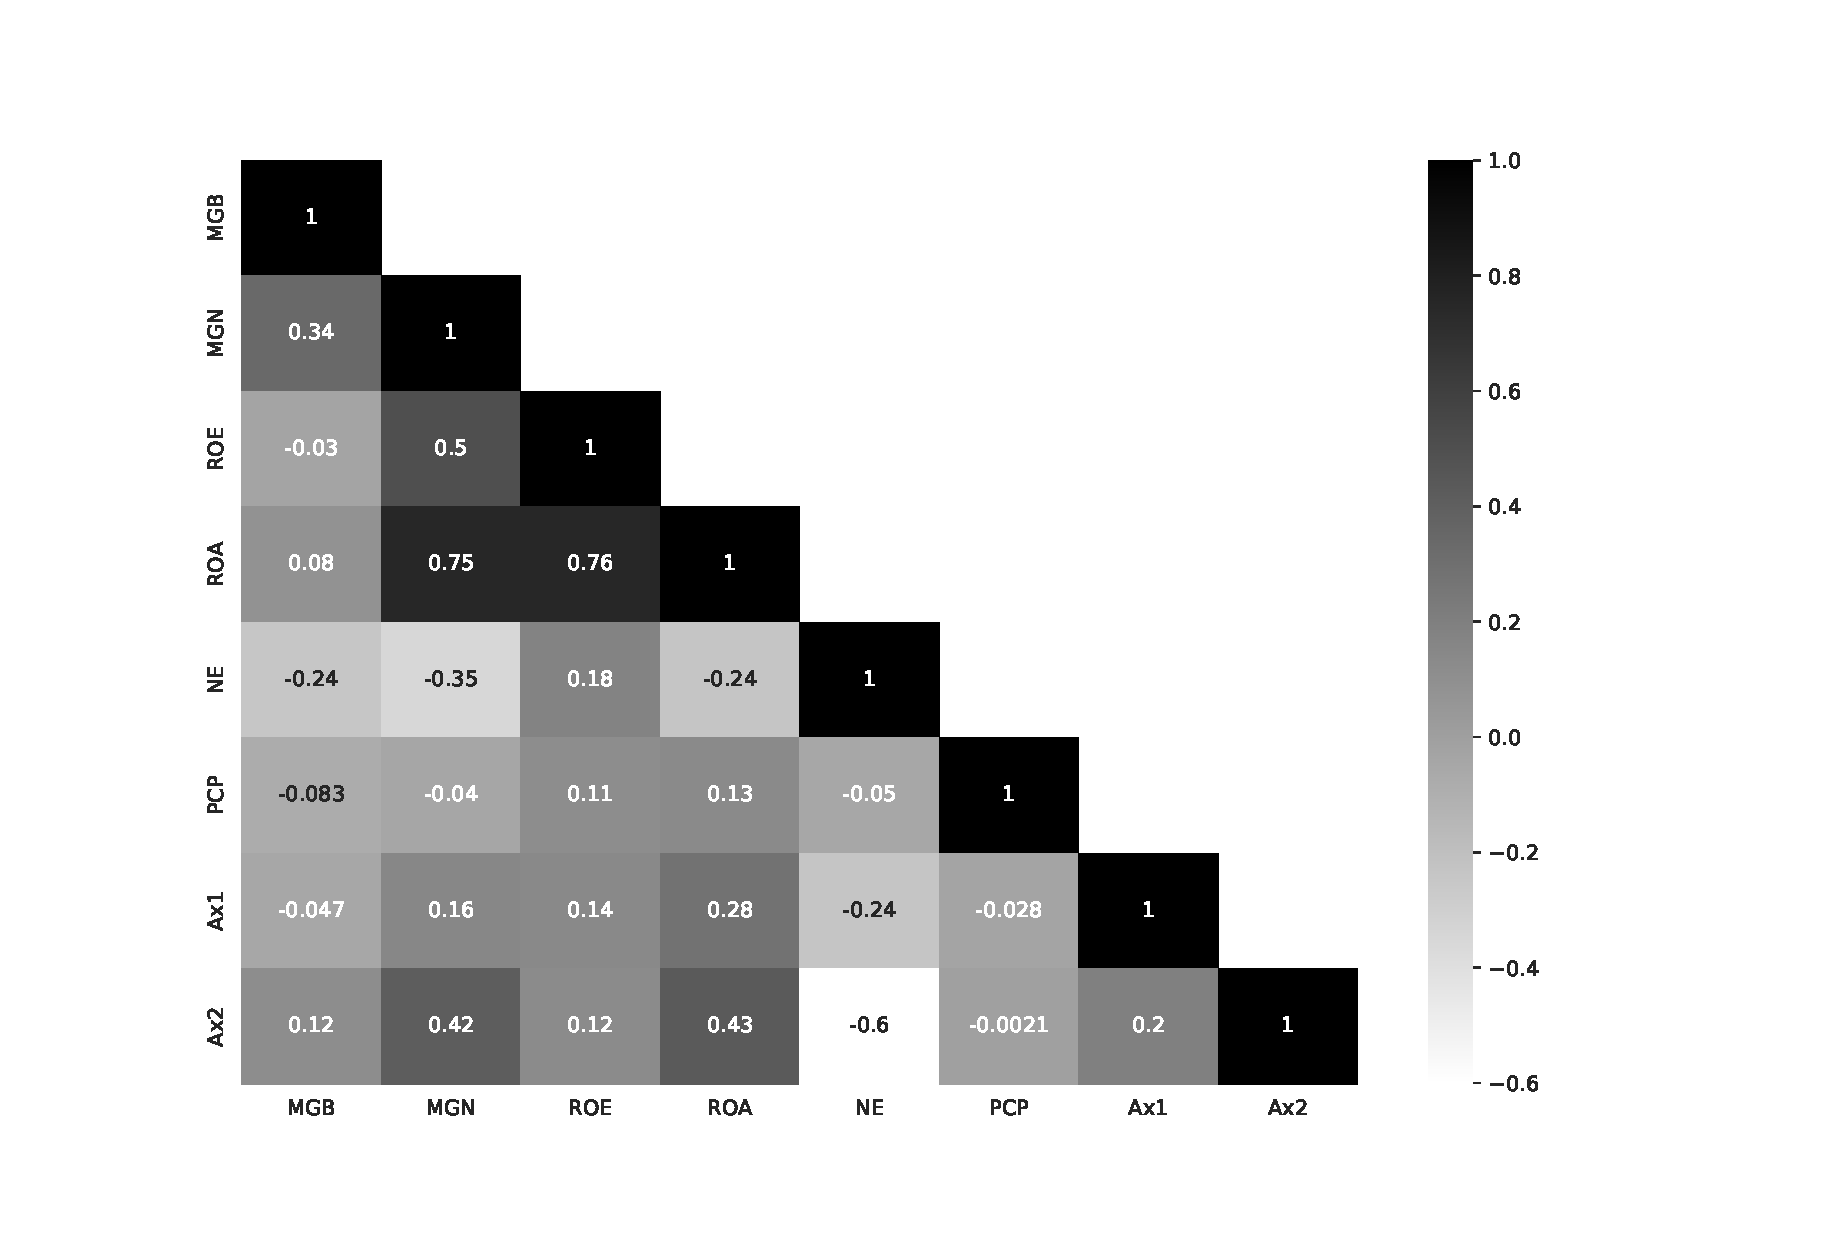
\includegraphics[scale=0.38]{Matrix.eps}
\end{figure}

There are a relationship among the variables.






\begin{table*}[b]	
\ContinuedFloat
    \centering
\caption{Model performance with one year of lag}
\begin{tabularx}{\linewidth}{lCCCCCCl}
\toprule
 \multicolumn{1}{c}{}& \multicolumn{2}{c}{Logistic Regression} & \multicolumn{2}{c}{Decision Tree} & \multicolumn{2}{c}{Multilayer Perceptron}\\
\cmidrule(lr){2-3}   \cmidrule(lr){4-5}  \cmidrule(lr){6-7} \\
 & Default & No-deafult & Default & No-default & No-default & Default \\
\midrule
precision & 1.00 & 0.53 & 0.79 & 0.58 & 0.00 & 0.49 \\
recall & 0.12 & 1.00 & 0.38 & 0.90 & 0.00 & 1.00 \\
f1-score & 0.22 & 0.69 & 0.51 & 0.71 & 0.00 & 0.66 \\
support & 40.00 & 39.00 & 40.00 & 39.00 & 40.00 & 39.00 \\
\bottomrule
\end{tabularx}
\end{table*}





% word with c and l
\begin{table*}[b]
\setlength\tabcolsep{15pt}
\ContinuedFloat
    \centering
\caption{Model performance with one year of lag}
\begin{tabular*}{\linewidth}{@{}*{7}{L}} 
\toprule
 &  & \multicolumn{5}{c}{Grouped by event} \\
 &  & Missing & Overall & 0.0 & 1.0 & P-Value \\
\midrule
n &  &  & 16806 & 16488 & 318 &  \\
\multirow{4}*{time-event, n (\%)} & 0.0 & 0 & 16488 (98.11) & 16488 (100.00) &  & \< 0.001 \\
 & 2017.0 &  & 99 (0.59) &  & 99 (31.13) &  \\
 & 2018.0 &  & 96 (0.57) &  & 96 (30.19) &  \\
 & 2019.0 &  & 123 (0.73) &  & 123 (38.68) &  \\
MGB, median [Q1,Q3] &  & 0 & 0.31 [0.18,0.56] & 0.32 [0.18,0.56] & 0.26 [0.14,0.41] & <0.001 \\
MGN, median [Q1,Q3] &  & 0 & 0.03 [0.00,0.08] & 0.03 [0.00,0.08] & -0.02 [-0.18,0.03] & <0.001 \\
ROE, median [Q1,Q3] &  & 0 & 0.07 [0.01,0.16] & 0.07 [0.01,0.16] & 0.01 [-0.18,0.09] & <0.001 \\

ROA, median [Q1,Q3] &  & 0 & 0.03 [0.00,0.06] & 0.03 [0.00,0.07] & -0.01 [-0.09,0.01] & <0.001 \\
NE, median [Q1,Q3] &  & 0 & 0.53 [0.32,0.72] & 0.52 [0.32,0.72] & 0.74 [0.59,0.88] & <0.001 \\
PCP, median [Q1,Q3] &  & 0 & 0.75 [0.45,0.98] & 0.75 [0.45,0.98] & 0.53 [0.28,0.87] & <0.001 \\
Ax1, median [Q1,Q3] &  & 0 & 0.22 [0.04,0.43] & 0.22 [0.04,0.43] & 0.09 [-0.08,0.28] & <0.001 \\
Ax2, median [Q1,Q3] &  & 0 & 0.19 [0.04,0.40] & 0.19 [0.05,0.40] & 0.04 [-0.12,0.18] & <0.001 \\
\multirow[t]{20}*{Sector, n (\%)} & Actividades artísticas, de entretenimiento y recreación & 0 & 88 (0.52) & 86 (0.52) & 2 (0.63) & <0.001 \\
 & Actividades de atención de la salud humana y de asistencia social &  & 64 (0.38) & 63 (0.38) & 1 (0.31) &  \\
 & Actividades de organizaciones y entidades extraterritoriales &  & 3 (0.02) & 3 (0.02) &  &  \\
 & Actividades de servicios administrativos y de apoyo &  & 646 (3.84) & 632 (3.83) & 14 (4.40) &  \\
 & Actividades financieras y de seguros &  & 474 (2.82) & 473 (2.87) & 1 (0.31) &  \\
 & Actividades inmobiliarias &  & 1449 (8.62) & 1443 (8.75) & 6 (1.89) &  \\
 & Actividades profesionales,  científicas y técnicas &  & 1142 (6.80) & 1127 (6.84) & 15 (4.72) &  \\
 & Administración pública y defensa; planes de seguridad social de afiliación obligatoria &  & 4 (0.02) & 4 (0.02) &  &  \\
 & Agricultura, ganadería, caza, silvicultura y pesca &  & 1012 (6.02) & 990 (6.00) & 22 (6.92) &  \\
 & Alojamiento y servicios de comida &  & 363 (2.16) & 349 (2.12) & 14 (4.40) &  \\
 & Comercio al por mayor y al por menor; reparación de vehículos automotores y motocicletas &  & 5288 (31.46) & 5201 (31.54) & 87 (27.36) &  \\
 & Construcción &  & 2238 (13.32) & 2190 (13.28) & 48 (15.09) &  \\
 & Distribución de agua; evacuación y tratamiento de aguas residuales, gestión de desechos y actividades de saneanmiento ambiental &  & 28 (0.17) & 27 (0.16) & 1 (0.31) &  \\
 & Educación &  & 87 (0.52) & 86 (0.52) & 1 (0.31) &  \\
 & Explotación de minas y canteras &  & 282 (1.68) & 277 (1.68) & 5 (1.57) &  \\
 & Industrias manufacturetas &  & 2735 (16.27) & 2647 (16.05) & 88 (27.67) &  \\
 & Información y comunicaciones &  & 464 (2.76) & 456 (2.77) & 8 (2.52) &  \\
 & Otras actividades de servicios &  & 115 (0.68) & 114 (0.69) & 1 (0.31) &  \\
 & Suministro de electricidad, gas, vapor y aire acondicionado &  & 10 (0.06) & 10 (0.06) &  &  \\
 & Transporte y almacenamiento &  & 314 (1.87) & 310 (1.88) & 4 (1.26) &  \\
\cline{1-7}
\bottomrule
\end{tabular*}
\end{table*}





\section{Appendix}
The financial ratios used were:

\begin{itemize}
\item new
\end{itemize}


  




were






\newpage
\printbibliography





\end{document}